\documentclass[tikz,border=8pt]{standalone}
\usepackage{newtxtext,newtxmath}
\usetikzlibrary{arrows.meta,calc,fit,positioning}

\definecolor{axisx}{HTML}{DCEBFA}
\definecolor{axisy}{HTML}{DDF3E4}
\definecolor{axisz}{HTML}{FCE8D5}
\definecolor{groupborder}{HTML}{7A8793}
\definecolor{labelgray}{HTML}{4A5560}

\begin{document}
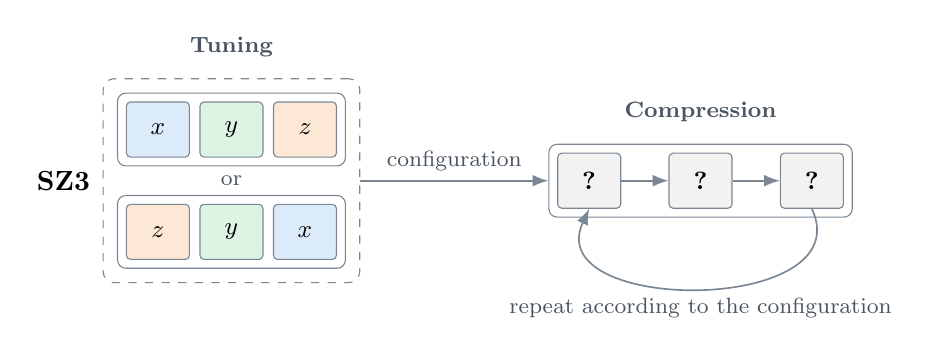
\begin{tikzpicture}[
round/.style={draw=groupborder,rounded corners=1.5pt,minimum width=8mm,minimum height=7mm,font=\small},
group/.style={draw=groupborder,rounded corners=3pt,inner sep=3pt},
note/.style={font=\footnotesize,text=labelgray},
flow/.style={-{Latex[length=2mm]},draw=groupborder,line width=.6pt},
stage/.style={font=\bfseries\footnotesize,text=labelgray}
]
\node[font=\bfseries] at (-1.2,0) {SZ3};

\node[round,fill=axisx](c1)at(0,.65){$x$};
\node[round,fill=axisy,right=1.2mm of c1](c2){$y$};
\node[round,fill=axisz,right=1.2mm of c2](c3){$z$};
\node[group,fit=(c1)(c3)](cg1){};
\node[round,fill=axisz](c4)at(0,-.65){$z$};
\node[round,fill=axisy,right=1.2mm of c4](c5){$y$};
\node[round,fill=axisx,right=1.2mm of c5](c6){$x$};
\node[group,fit=(c4)(c6)](cg2){};
\node[note]at($(cg1.south)!.5!(cg2.north)$){or};
\node[draw=groupborder,dashed,rounded corners=4pt,fit=(cg1)(cg2),inner sep=5pt](tuning){};
\node[stage,above=1.5mm of tuning]{Tuning};

\node[round,fill=black!5,font=\bfseries\small,right=25mm of tuning](q1){?};
\node[round,fill=black!5,font=\bfseries\small,right=6mm of q1](q2){?};
\node[round,fill=black!5,font=\bfseries\small,right=6mm of q2](q3){?};
\node[group,fit=(q1)(q3)](cycle){};
\node[stage,above=1.5mm of cycle]{Compression};

\draw[flow](tuning.east)--node[above,note]{configuration}(cycle.west);
\draw[flow](q1.east)--(q2.west);
\draw[flow](q2.east)--(q3.west);
\draw[flow](q3.south)to[out=-65,in=-115,looseness=1.35]node[below,note]{repeat according to the configuration}(q1.south);
\end{tikzpicture}
\end{document}
